\chapter{multirobot\_map\_merge}
\label{chap:map_merge-doc}

\section{Package Summary}

Merging multiple maps with knowledge of the initial relative positions of robots.

\begin{itemize}
    \item Maintainer status: developed
    \item Maintainer: Jiri Horner \textless laeqten AT gmail DOT com\textgreater
    \item Author: Jiri Horner \textless laeqten AT gmail DOT com\textgreater
    \item License: BSD
    \item Source: git \url{https://github.com/hrnr/m-explore.git} (branch: master)
\end{itemize}

\section{Overview}

This package provides global map for multiple robots. It can merge maps from arbitrary number of robots. It expects maps from individual robots as ROS topics. If your run multiple robots under the same ROS master then \texttt{multirobot\_map\_merge} will probably work for you out-of-the-box. It is also very easy to setup an simulation experiment.

\begin{figure}
    \centering
    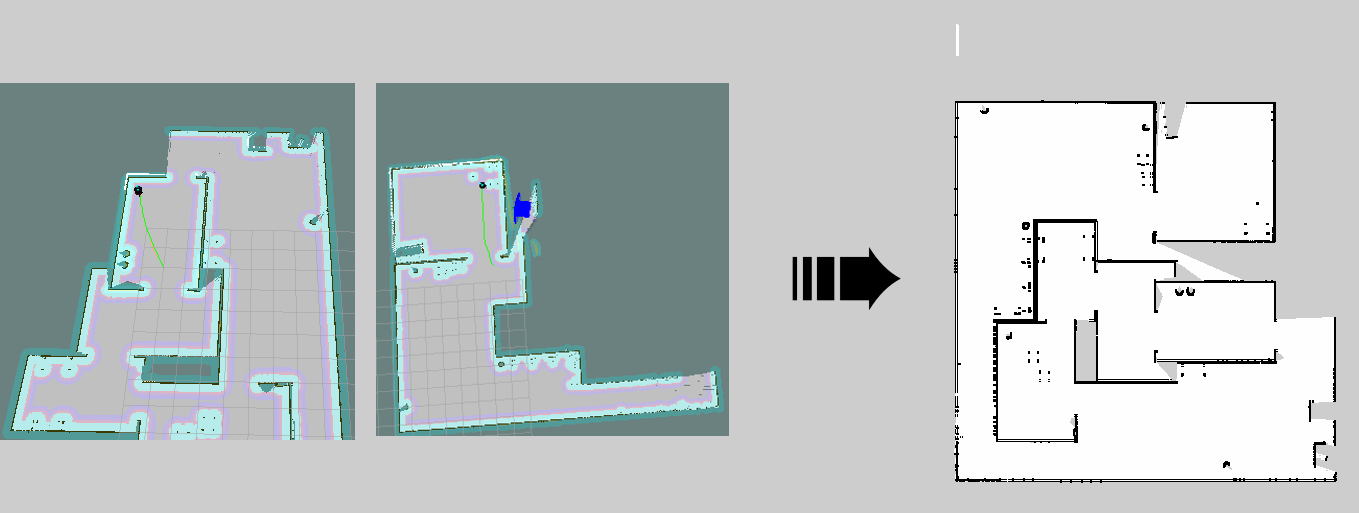
\includegraphics[width=4.53in]{../img/map_merge_cover.png}
    \caption[The merged map for $2$ robots.]{Output of \texttt{multirobot\_map\_merge}, map merging node for \gls{ROS}. The merged map for $2$ robots. Robots in the environment visualised on the left, merged map on the right.}
    \label{fig:mapmergecover}
\end{figure}

If your run your robots under multiple ROS masters you need to run your own way of communication between robots and provide maps from robots on local topics (under the same master). Also if you want to distribute merged map back to robots your communication must take care of it.

%<<Youtube(8Adrn29BVbM&rel=0)>>

\texttt{multirobot\_map\_merge} does not depend on any particular communication between robots.

\section{Architecture}

\texttt{multirobot\_map\_merge} finds robot maps dynamically and new robots can be added to system at any time.

\begin{figure}
    \centering
    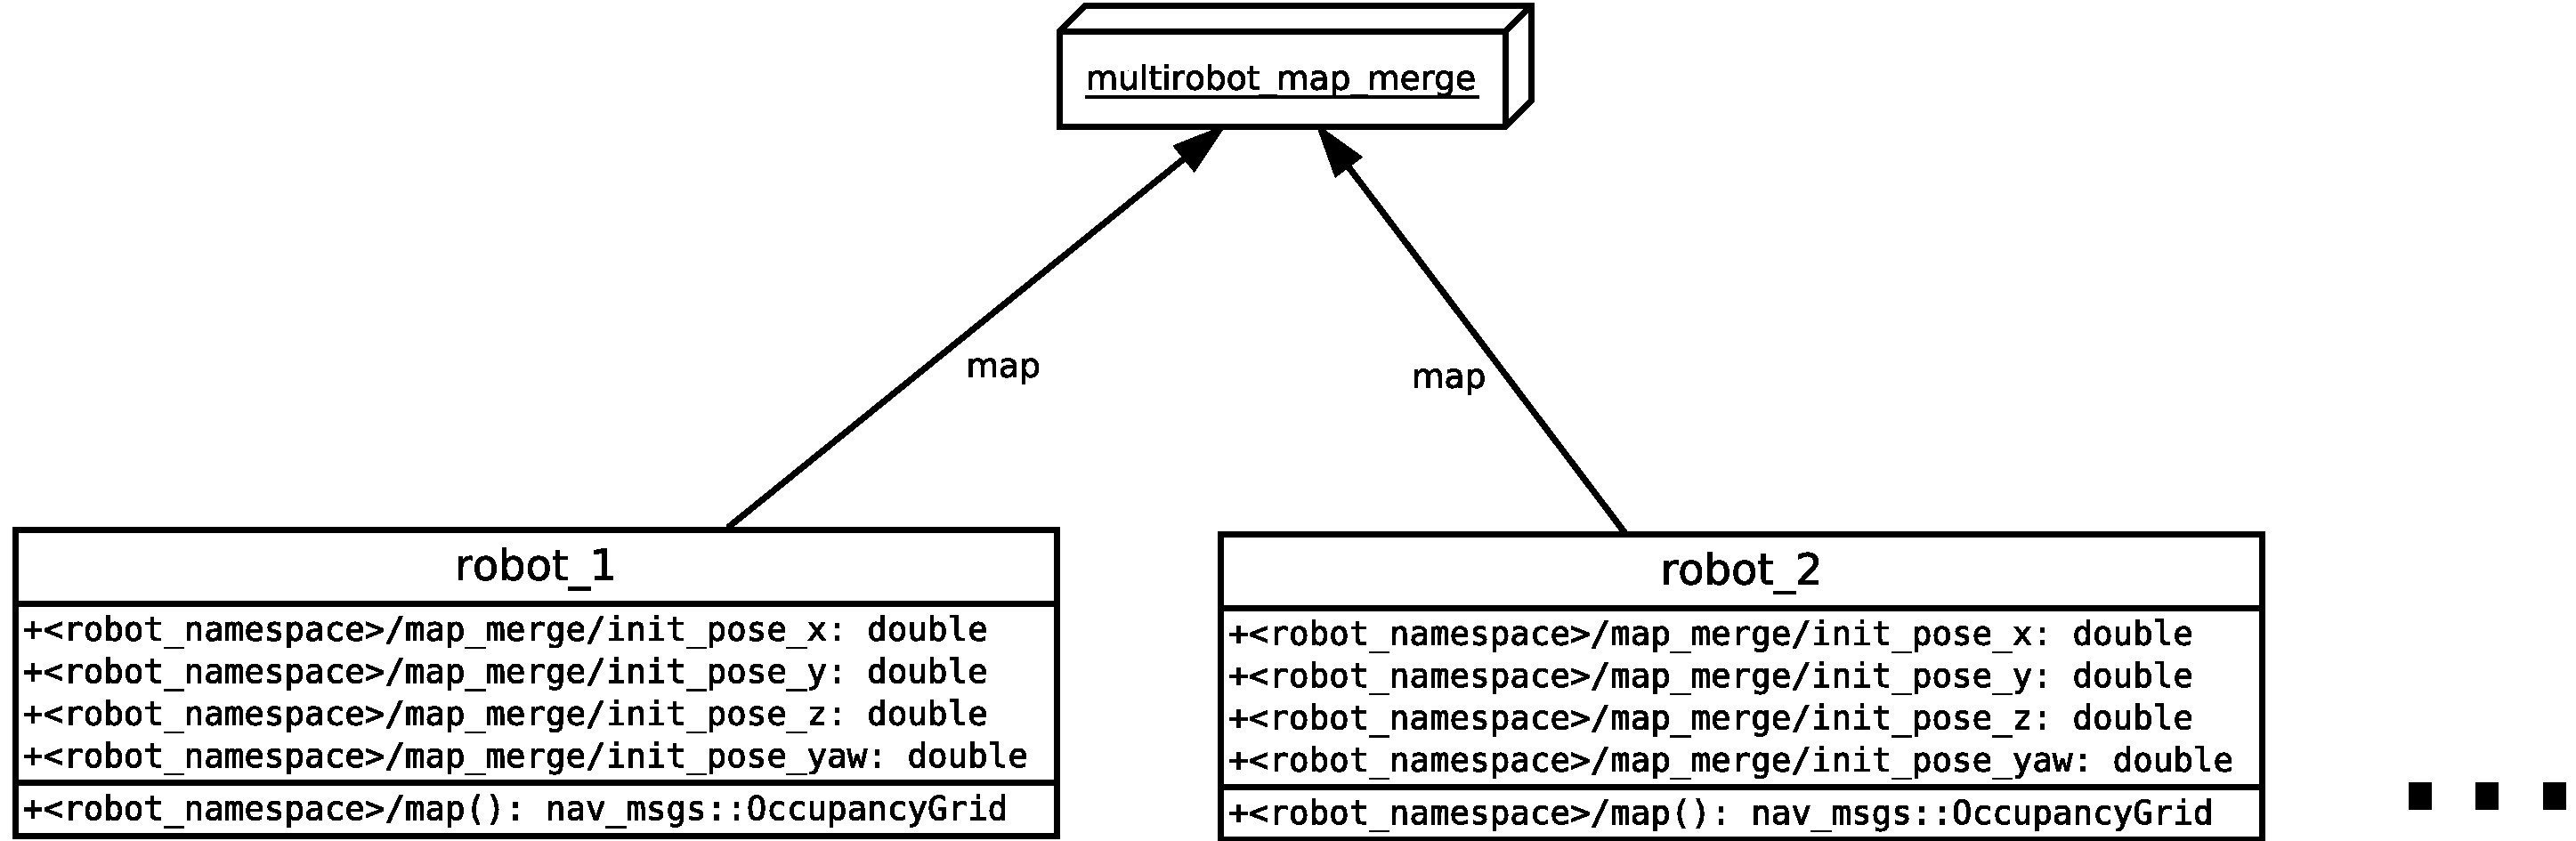
\includegraphics[width=\textwidth]{../img/map_merge_architecture.pdf}
    \caption[Architecture of \texttt{multirobot\_map\_merge}.]{Architecture of \texttt{multirobot\_map\_merge}, proposed map merging node for \gls{ROS}.}
    \label{fig:mapmergearchitecture}
\end{figure}

To make this dynamic behaviour possible there are some constrains placed on robots. First all robots must publish map under \texttt{<robot\_namespace>/map}, where topic name (\texttt{map}) is configurable, but must be same for all robots. For each robot \texttt{<robot\_namespace>} will be of cause different.

This node support merging maps with known initial positions of the robots or without. See below for details.

\section{Merging modes}
\label{sec:mergingmodes}

Two merging modes are currently supported as orthogonal options. If you know initial positions of robots you may preferably use the first mode and get exact results (rigid transformation will be computed according to initial positions). If you don't know robot's starting points you are still able to use the second mode where transformation between grids will be determined using heuristic algorithm. You can choose between these two modes using the \texttt{known\_init\_poses} parameter.

\subsection{merging with known initial positions}

This is preferred mode whenever you are able to determine exact starting point for each robot. You need to provide initial position for each robot. You need to provide set of \texttt{<robot\_namespace>/map\_merge/init\_pose} parameters. These positions should be in \texttt{world\_frame}. See Section~\ref{sec:rosapi}.

In this merging these parameters are mandatory. If any of the required parameters is missing robot won't be considered for merging (you will get warning with name of affected robot).

\subsection{merging without known initial positions}

If you can't provide initial poses for robots this mode has minimal configuration requirements. You need to provide only map topic for each robot. Transformation between grids is estimated by feature-matching algorithm and therefore requires grids to have sufficient amount of overlapping space to make a high-probability match. If grids don't have enough overlapping space to make a solid match, merged map can differ greatly from physical situation.

Estimating transforms between grids is cpu-intesive so you might want to tune \texttt{estimation\_rate} parameter to run re-estimation less often if it causes any troubles.

\section{ROS API}
\label{sec:rosapi}

\subsection{map\_merge}

Provides map merging services offered by this package. Dynamically looks for new robots in the system and merges their maps.

\subsubsection{Subscribed Topics}
  \ROStopic{<robot\_namespace>/map}{nav\_msgs/OccupancyGrid}{Local map for specific robot.}

  \ROStopic{<robot\_namespace>/map\_updates}{map\_msgs/OccupancyGridUpdate}{Local map updates for specific robot. Most of the \texttt{nav\_msgs/OccupancyGrid} sources (mapping algorithms) provides incremental map updates via this topic so they don't need to send always full map. This topic is optional. If your mapping algorithm does not provide this topic it is safe to ignore this topic. However if your mapping algorithm does provide this topic, it is preferable to subscribe to this topic. Otherwise map updates will be slow as all partial updates will be missed and map will be able to update only on full map updates.}

\subsubsection{Published Topics}
  \ROStopic{map}{nav\_msgs/OccupancyGrid}{Merged map from all robots in the system.}

\subsubsection{Parameters}
\paragraph{Robot Parameters}

Parameters that should be defined in the namespace of each robot if you want to use merging with known initial poses of robots (\texttt{known\_init\_poses} is \texttt{true}). Without these parameters robots won't be considered for merging. If you can't provide these parameters use merging without known initial poses. See Section~\ref{sec:mergingmodes}

    \ROSparam{<robot\_namespace>/map\_merge/init\_pose\_x}{<no\_default>}{double}{\texttt{x} coordinate of robot initial position in \texttt{world\_frame}. Should be in meters. It does not matter which frame you will consider global (preferably it should be different from all robots frames), but relative positions of robots in this frame must be correct.}

    \ROSparam{<robot\_namespace>/map\_merge/init\_pose\_y}{<no\_default>}{double}{\texttt{y} coordinate of robot initial position in \texttt{world\_frame}.}

    \ROSparam{<robot\_namespace>/map\_merge/init\_pose\_z}{<no\_default>}{double}{\texttt{z} coordinate of robot initial position in \texttt{world\_frame}.}

    \ROSparam{<robot\_namespace>/map\_merge/init\_pose\_yaw}{<no\_default>}{double}{\texttt{yaw} component of robot initial position in \texttt{world\_frame}. Represents robot rotation in radians.}

\paragraph{Node Parameters}

Parameters that should be defined in the namespace of this node.

    \ROSparam{\~{}robot\_map\_topic}{map}{string}{Name of robot map topic without namespaces (last component of topic name). Only topics with this name will be considered when looking for new maps to merge. This topics may be subject to further filtering (see below).}

    \ROSparam{\~{}robot\_map\_updates\_topic}{map\_updates}{string}{Name of robot map updates topic of \texttt{map\_msgs/OccupancyGridUpdate} without namespaces (last component of topic name). This topic will be always subscribed in the same namespace as \texttt{robot\_map\_topic}. You'll likely need to change this only when you changed \texttt{robot\_map\_topic}. These topics are never considered when searching for new robots.}

    \ROSparam{\~{}robot\_namespace}{<empty string>}{string}{Fixed part of robot map topic. You can employ this parameter to further limit which topics will be considered during dynamic lookup for robots. Only topics which contain (anywhere) this string will be considered for lookup. Unlike \texttt{robot\_map\_topic} you are not limited by namespace logic. Topics will be filtered using text-based search. Therefore \texttt{robot\_namespace} does not need to be ROS namespace, but can contain slashes etc. This must be common part of all robots map topics name (all robots for which you want to merge map).}

    \ROSparam{\~{}known\_init\_poses}{true}{bool}{Selects between merging modes. \texttt{true} if merging with known initial positions. See Section~\ref{sec:mergingmodes}}

    \ROSparam{\~{}merged\_map\_topic}{map}{string}{Topic name where merged map will be published.}

    \ROSparam{\~{}world\_frame}{world}{string}{Frame id (in \href{http://wiki.ros.org/tf}{tf} tree) which will be assigned to published merged map. This should be frame where you specified robot initial positions.}

    \ROSparam{\~{}merging\_rate}{4.0}{double}{Rate in Hz. Basic frequency on which this node discovers merges robots maps and publish merged map. Increase this value if you want faster updates.}

    \ROSparam{\~{}discovery\_rate}{0.05}{double}{Rate in Hz. Frequency on which this node discovers new robots. Increase this value if you need more agile behaviour when adding new robots. Robots will be discovered sooner.}

    \ROSparam{\~{}estimation\_rate}{0.5}{double}{Rate in Hz. This parameter is relevant only when merging without known positions, see Section~\ref{sec:mergingmodes}. Frequency on which this node re-estimates transformation between grids. Estimation is cpu-intensive, so you may wish to lower this value.}

    \ROSparam{\~{}estimation\_confidence}{1.0}{double}{Relevant only when merging without known positions, see Section~\ref{sec:mergingmodes}. Confidence according to probabilistic model for initial positions estimation. Default value 1.0 is suitable for most applications, increase this value for more confident estimations. Number of maps included in the merge may decrease with increasing confidence. Generally larger overlaps between maps will be required for map to be included in merge. Good range for tuning is $[1.0, 2.0]$.}

\section{Acknowledgements}

This package was developed as part of my bachelor thesis at \href{http://www.mff.cuni.cz/to.en/}{Charles University} in Prague.

Idea for dynamic robot discovery is from \href{http://wiki.ros.org/map_merging}{map\_merging} package from Zhi Yan. Merging algorithm and configuration are different.
